% -*- TeX:de -*-
\NeedsTeXFormat{LaTeX2e}
\documentclass[12pt,a4paper]{article}
\usepackage[german]{babel} % german text
\usepackage[DIV12]{typearea} % size of printable area
\usepackage[T1]{fontenc} % font encoding
%\usepackage[latin1]{inputenc} % most likely on Windows
\usepackage[utf8]{inputenc} % probably on Linux
\usepackage{multicol}

% PLOTTING
\usepackage{pgfplots} 
\usepackage{pgfplotstable}
\usepackage{url}
\usepackage{graphicx} % to include images
\usepackage{tikz}
\usepackage{subfigure} % for creating subfigures
\usepackage{amsmath} % a bunch of symbols
\usepackage{amssymb} % even more symbols
\usepackage{booktabs} % pretty tables
\usepackage{makecell} % multi row table heading

% a floating environment for circuits
\usepackage{float}
\usepackage{caption}

%\newfloat{circuit}{tbph}{circuits}
%\floatname{circuit}{Schaltplan}

% a floating environment for diagrams
%\newfloat{diagram}{tbph}{diagrams}
%\floatname{diagram}{Diagramm}
\pgfplotsset{compat=1.8}
\selectlanguage{german} % use german

\begin{document}

%%%%%%% DECKBLATT %%%%%%%
\thispagestyle{empty}
			\begin{center}
			\Large{Fakultät für Physik}\\
			\end{center}
\begin{verbatim}


\end{verbatim}
							%Eintrag des Wintersemesters
			\begin{center}
			\textbf{\LARGE SS 14}
			\end{center}
\begin{verbatim}


\end{verbatim}
			\begin{center}
			\textbf{\LARGE{Physikalisches Praktikum\\ für das Bachelorstudium}}
			\end{center}
\begin{verbatim}




\end{verbatim}

			\begin{center}
			\textbf{\LARGE{PROTOKOLL}}
			\end{center}
			
\begin{verbatim}

\end{verbatim}

			\begin{flushleft}
			\textbf{\Large{Experiment (Nr., Titel): PS1 - Schwingungen 1}\\
							%Experiment Nr. und Titel statt den Punkten eintragen
			\LARGE{PS1}}	
			\end{flushleft}

\begin{verbatim}

\end{verbatim}	
							%Eintragen des Abgabedatums, oder des Erstelldatums des Protokolls
			\begin{flushleft}
			\textbf{\Large{Datum:}} \Large{05.06.2014}
			\end{flushleft}
			
\begin{verbatim}
\end{verbatim}
							%Namen der Protokollschreiber
		\begin{flushleft}
			\textbf{\Large{Namen:}} \Large{Patrick Braun, Johannes Kurz}
			\end{flushleft}

\begin{verbatim}


\end{verbatim}
							%Kurstag und Gruppennummer, zb. Fr/5
			\begin{flushleft}
			\textbf{\Large{Kurstag/Gruppe:}} \Large{DO/4}
			\end{flushleft}

\begin{verbatim}

\end{verbatim}
							%Name des Betreuers, das Praktikum betreute.
			\begin{flushleft}
			\LARGE{\textbf{Betreuer:}}	\Large{Wilhelm Markowitsch}	
			\end{flushleft}

%%%%%%% DECKBLATT ENDE %%%%%%%
\pagebreak
\setlength{\columnsep}{20pt}
\begin{multicols}{2}

%%%%%%%%%%%%%%%%%%%%%%%%%%%%%%%%%%%%%%%%%%%%%%%%

%\begin{figure}[H]
%	\centering
%	\includegraphics[scale=0.35]{./data/beugung.png}
%	\caption{Beugungsmuster Einzelspalt (echtes Foto; schwarz durch weiß ersetzt)}
%	\label{fig:beugungsmuster}
%\end{figure}


%\begin{figure}[H]
%	\centering
%	\pgfplotstabletypeset[
%			columns={abstand, n},
%			col sep=&,
%			columns/abstand/.style={precision=2, zerofill, column name=\makecell{$Abstand$\\$(\pm 0.05)[mm]$} }, 
%			columns/n/.style={column name=\makecell{$n$\\$(Ordnung)$}, precision=0},
%			every head row/.style={before row=\hline,after row=\hline\hline},
%			every last row/.style={after row=\hline},
%			every first column/.style={column type/.add={|}{} },
%			every last column/.style={column type/.add={}{|} }
%			]{
%			abstand & n
%			12.9 & 1
%			24.45 & 2
%			37.40 & 3
%			49.35& 4
%			62.45 & 5
%			74.45 & 6
%			87.45 & 7
%			100.25 & 8
%			
%			}
%	\caption{Messwerte Einzelspalt}
%	\label{tab:werte_einzelspalt}
%\end{figure}


%%%%%%%%%%%%%%%%%%%%%%%%%%%%%%%%%%%%%%%%%%%%%%%%
%%%%%%%%%%%%%%%%%%%%%%%%%%%%%%%%%%%%%%%%%%%%%%%%


\section{Schwingungen 1}
In PS1 werden mechanische Oszillatoren auf ihre Eigenschaften untersucht.\\
Im Detail werden ein Drehpendel, ein gekoppeltes Pendel und die Dopplerverschiebung betrachtet. Dabei werden gedämpfte Schwingungen, auch getriebene sowie Schwebungen (Kopplung, Dopplereffekt) untersucht.
%%%%%%%%%%%%%%%%%%%%%%%%%%%%%%%%%%%%%%%%%%%%%%%%%%%%%%%%%%%%%%%%%%%%%%%
\section{Grundlagen:}
Die Bewegungsgleichung, die einen gedämpften harmonischen Oszillator beschreibt ist klassisch gegeben durch:
$$m  \ddot{x} + k \dot{x} + D x = 0$$
$m$... Masse\\
$k$... Reibungszahl\\
$D$... Federkonstante\\

\noindent Die Lösung der Gleichung für den ungedämpften (k=0) harmonischen Oszillator sind die Winkelfunktionen:
$$x(t) = A \cdot cos(\omega t + \phi)$$
Dabei ist \textbf{A} die Amplitude, \textbf{$\omega$} die Kreisfrequenz, \textbf{t} die Zeit und \textbf{$\phi$} die Phase, also die Auslenkung, mit der die Schwingung begonnen hat (zu t=0).\\
Betrachtet man nun eine gedämpfte Schwingung ergibt sich als Lösung ein zusätzlicher zeitabhängiger Dämpfungsterm: 
$$x(t) = A \cdot e^{- \delta t} \cdot cos(\omega t + \phi)$$ 
Hierbei ist $\delta$ die Dämpfungskonstante welche vom Material (z.B. Luft, Eisen) und anderen Bedingungen abhängt (z.B. Kugellager, Reibung etc.).\\
Der Dämpfungskoeffizient  wird durch das logarithmische Dämpfungsdekrement $\Lambda$ berechnet:
$$\Lambda = ln \frac{x(T_1)}{x(T_2)} = \delta T$$
Dabei wird die Änderung der Amplitude bei aufeinander folgenden Perioden betrachtet ($\frac{x(T_1)}{x(T_2)} = e^{\delta T}$).\\

\noindent Eine reale Schwingung ist nie völlig ungedämpft. Die Frequenz, mit der ein ungedämpfter Oszillator (theoretisch) schwingen würde, heißt \textbf{Eigenfrequenz} und wird im im Folgenden als $\omega_0$ bezeichnet.\\
Die Eigenfrequenz wird bei bekanntem $\delta$ über folgende Relation berechnet:
%$$ \omega_0 = \sqrt{\frac{2\cdot \delta \omega}{tan \phi} + \omega^2 }$$
$$\omega = \sqrt{\omega_0^2 - \delta^2}$$
Eine zweite Möglichkeit die Eigenfrequenz zu bestimmen, ist es, die Resonanzkurve einer erzwungenen Schwingung zu ermitteln und die Halbwertsbreite des Amplitudenpeaks (bei $\frac{A_{max}}{\sqrt{2}}$ ) zu messen (vgl. [1](9, p.6)).\\
Wird ein Oszillator durch eine periodische Kraft getrieben (rechts vom "$=$" kommt eine zeitabhängige Kraft $F(t)$ dazu), die genau, oder fast genau, mit der Eigenfrequenz geht, gibt es Resonanz. Der Oszillator beginnt also immer stärker zu schwingen. Wäre er ungedämpft, würde sich so seine Amplitude (und auch seine Energie) nach $\infty$ steigern lassen. Real kann dies eben nicht passieren.\\
Wächst die Amplitude eines schwingendes System jedoch über alle (mechanischen und baulichen) Grenzen hinaus, sodass das System zerstört wird, spricht man von einer Resonanzkatastrophe.\\
Ein weiteres Maß für einen Oszillator ist der Gütefaktor Q. Dieser ist definiert als:
$$Q = \frac{\omega_0}{2\delta} = \frac{\omega_0}{\Delta \omega}$$






\subsection{Gekoppelte Pendel}
Bei einem gekoppelten Pendel beeinflussen sich wechselseitig zwei Pendel welche miteinander verbunden sind. In Abbildung \ref{fig:gekoppelt_skizze} sind die wesentlichen Parameter der Kopplung zu sehen.

\begin{figure}[H]
	\centering
	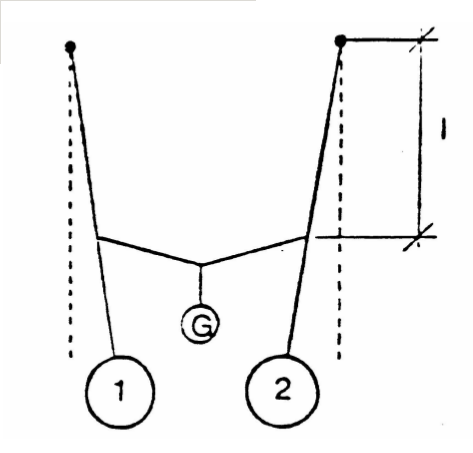
\includegraphics[scale=0.45]{./figure/skizze_kopplung.png}
	\caption{Skizze eines gekoppelten Pendels [1](Abb.7, p.9)}
	\label{fig:gekoppelt_skizze}
\end{figure}
\noindent Die Kopplungslänge \textbf{l} und das Gewicht \textbf{G} beeinflussen die Schwingung des Gesamtsystems. Je nach Anfangsbedingungen kann man drei Sonderfälle unterscheiden:\\
\begin{itemize}
	\item  \textbf{Gleichsinnige Schwingung} \\ beide schwingen parallel mit $\omega_0$, gleicher Phase und gleicher Amplitude
	\item  \textbf{Gegensinnige Schwingung} \\ beide Pendel schwingen mit einer (kopplungsabhängig) höheren Frequenz $\omega_1$, wobei ihre Amplituden gleich sind, sie jedoch einen Phasenversatz von $\phi = \pi$ haben.
	\item  \textbf{Schwebungsfall} \\ zu Beginn schwingt nur ein Pendel mit einer Frequenz $\omega_2$, das zweite ruht. Die gesamte Energie des schwingenden wird langsam auf das ruhende übertragen; dieses beginnt zu schwingen, bis es die ursprüngliche Amplitude des ersten Pendels hat und dieses ruht und der Kreislauf beginnt von vorne.\\
	(der Verlauf der Amplitudenänderung ist periodisch mit $\omega_S$)
\end{itemize}

\noindent Diese Eigenfrequenzen des Systems ergeben sich aus der Lösung der Bewegungsgleichung für gekoppelte Pendel. Es werden 2 Oszillatoren sowie eine zusätzliche Rückstellkraft aus der Kopplung betrachtet.\\
$\omega_S$ und $\omega_2$ lassen sich auch aus den Eigenfrequenzen der gleich- sowie der gegensinnigen Schwingung berechnen:
$$\omega_S = \frac{\omega_1 - \omega_0}{2}$$
$$\omega_2 = \frac{\omega_1 +\omega_0}{2}$$

\noindent Der Kopplungsgrad \textbf{K} ist gegeben durch:
$$K = \frac{\omega_1^2 - \omega_0^2}{\omega_1^2 + \omega_0^2} =  \frac{2\omega_S \omega_2}{\omega_S^2 + \omega_2^2} $$

%%%%%%%%%%%%%%%%%%%%%%%%%%%%%%%%%%%%%%%%%%%%%
% TODO genauer ausformulieren + formeln
%%%%%%%%%%%%%%%%%%%%%%%%%%%%%%%%%%%%%%%%%%%%%

\subsection{Dopplerverschiebung einer bewegten Schallquelle}
Zur Bestimmung der Schallgeschwindigkeit anhand des Dopplereffekts wird in PS1 der Schwebungsfall 2er gekoppelter Oszillatoren (2 Lautsprecher bzw die von ihnen angeregte Luft) verwendet.\\
Der Dopplereffekt ist die Änderung einer Frequenz, wenn die erzeugende Quelle sich relativ zum Beobachter bewegt (klassisches Beispiel: Rettungswagen mit Blaulicht).\\
Anhand der Schwebungsdauer von zwei Schallquellen, die mit gleicher bekannter Frequenz betrieben werden (eine in Bewegung), und der Relativgeschwindigkeit, kann die Schallgeschwindigkeit in Luft durch folgende Relation bestimmt werden:
%$$c_{Luft} = \frac{v}{\frac{\nu}{\nu_0}-1}$$
$$\nu = \nu_0(1 + \frac{v}{c_{Luft}})$$
$\nu_0$ \ldots die Frequenz der Schallquelle\\ 
$\nu$ \ldots die durch den Dopplereffekt veränderte Frequenz\\
$v$ \ldots Bewegungsgeschwindigkeit\\
\\
Die Frequenzverschiebung durch den Dopplereffekt
$$\Delta \nu = \nu_0 - \nu$$
steht im Zusammenhang mit der Schwebungsdauer $T_S$ durch:
$$T_S = \frac{2 \pi}{\Delta \omega}= \frac{1}{\Delta \nu}$$
Durch einsetzen und umformen:
$$\frac{1}{T_S} = \frac{\nu_0}{c_{Luft}}\cdot v$$

Diese lineare Gleichung wird im Versuch benutzt, um aus mehreren Messungen von $T_S$ und $v$ den Anstieg $\frac{\nu_0}{c_{Luft}}$ zu ermitteln und daraus $c$.
%Trägt man $\Delta \nu / \nu_0$ gegen v auf, entspricht der Anstieg der Schallgeschwindigkeit.


\section{Versuchsaufbau:}
\subsection{Drehpendel:}

\subsection{Gekoppeltes Pendel:}

\subsection{Dopplerverschiebung einer bewegten Schallquelle:}
\pagebreak
%%%%%%%%%%%%%%%%%%%%%%%%%%%%%%%%%%%%%%%%%%%%%%%%%%%%%%%%%%%%%%%%%%%%%%%
\section{Resultate}
\subsection{Drehpendel}

\begin{figure}[H]
	\centering
	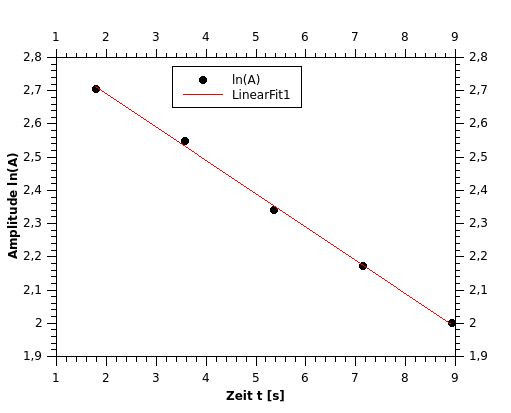
\includegraphics[scale=1.8]{./figure/Messung1_Daempfung_omega0.png}
	\caption{Bestimmung des Dämpfungskoeffizienten (Dämpfung mit 250mA)}
	\label{fig:daempfung_omega0_1}
\end{figure}

\noindent \textbf{Drehpendel - Dämpfung mit 250mA:}\\
Periodendauer (Mittel aus 5 Messungen):\\
$T = (1.7665 \pm 0.013)s$\\
$\Lambda = (-0.1718 \pm 0.0045)s$
$$\delta = \frac{ln(A)}{T} = (0.1003 \pm 0.0024)s^{-1}$$

$$\omega_{0 - 250mA}=(3.558 \pm 0.053)s^{-1}$$
Halbwertsbreite: 3.540 - 3.358:\\
$$\delta_{Halbwertsbreite} = (0.091 \pm 0.010)s^{-1}$$
$$Q_{250mA}=(17.74 \pm 0.50)$$


\end{multicols}
\begin{figure}[H]
	\centering
	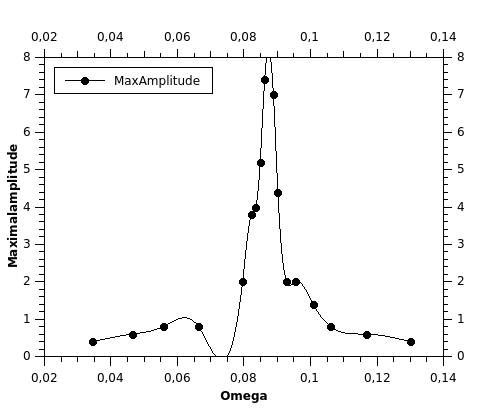
\includegraphics[scale=1.8]{./figure/Messung1_Resonanzkurve_250mA.png}
	\caption{Resonanzkurve (250mA)}
	\label{fig:resonanzkurve_250mA}
\end{figure}


\pagebreak
\begin{multicols}{2}

%\noindent \textbf{Drehpendel - Dämpfung mit 350mA:}\\
\begin{figure}[H]
	\centering
	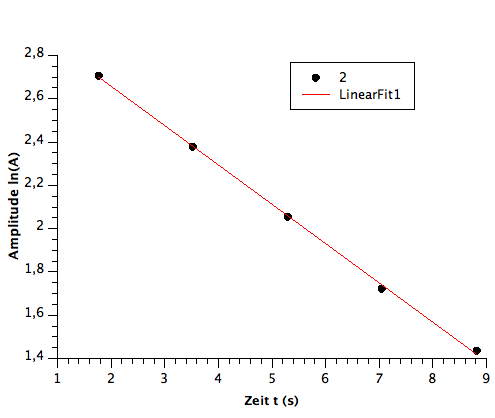
\includegraphics[scale=0.4]{./figure/Messung1_Daempfung_omega0-350mA.png}
	\caption{Bestimmung des Dämpfungskoeffizienten (Dämpfung mit 350mA)}
	\label{fig:daempfung_omega0_350mA}
\end{figure}

\noindent \textbf{Drehpendel - Dämpfung mit 350mA:}\\
\noindent Periodendauer (Mittel aus 5 Messungen):\\
$T = (1.7627 \pm 0.0063)s$\\
$\Lambda = (-0.3203 \pm 0.0048)s$
$$\delta = \frac{ln(A)}{T} = (0.1817 \pm 0.0026)s^{-1}$$

$$\omega_{0 - 350mA}=(3.569 \pm 0.026)s^{-1}$$
Halbwertsbreite: 3.59 - 3.26:\\
$$\delta_{Halbwertsbreite} = (0.165 \pm 0.010)s^{-1}$$
$$Q_{350mA}=(9.82 \pm 0.16)$$

% TODO grafik von Pats QTI 
%\begin{figure}[H]
%	\centering
%	%\includegraphics[scale=0.8]{./figure/Messung2_Daempfung_omega0.png}
%	\caption{Bestimmung des Dämpfungskoeffizienten Dämpfung 2 (350mA)}
%	\label{fig:daempfung_omega0_2}
%\end{figure}

\end{multicols}
\begin{figure}[H]
	\centering
	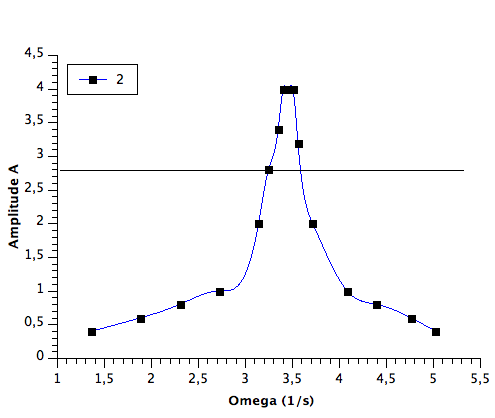
\includegraphics[scale=0.78]{./figure/Messung1_Resonanzkurve_350mA.png}
	\caption{Resonanzkurve (350mA)}
	\label{fig:resonanzkurve_350mA}
\end{figure}


\pagebreak
\begin{multicols}{2}




\subsection{Gekoppelte Pendel}

\noindent Kopplungslänge (beide Massen):\\
$l = (60.5 \pm 0.5 cm)$\\

\noindent Kopplungsmasse 1:\\
$m_1 = (504.3 \pm 0.1)g$

\noindent $\omega_{gk} = \omega_0 = (3.233 \pm 0.020)s^{-1}$\\
$\omega_{geg} = \omega_1 = (3.587\pm 0.034)s^{-1}$\\
$\omega_2 = (3.446 \pm 0.033)s^{-1}$\\
$\omega_{Schwebung}=\omega_S=(0.3638 \pm 0.0041)s^{-1}$

$$K_{\omega_0,\omega_1}=(0.105 \pm 0.012)$$
$$K_{\omega_2,\omega_S}=(0.1044 \pm 0.0026)$$
\\
\\
\noindent Kopplungsmasse 2:\\
$m_2 = (298.0 \pm 0.1)g$

\noindent $\omega_{gk} = \omega_0 = (3.232 \pm 0.018)s^{-1}$\\
$\omega_{geg} = \omega_1 = (3.466\pm 0.028)s^{-1}$\\
$\omega_2 = (3.341 \pm 0.019)s^{-1}$\\
$\omega_{Schwebung}=\omega_S=(0.25335 \pm 0.00013)s^{-1}$

$$K_{\omega_0,\omega_1}=(0.070 \pm 0.011)$$
$$K_{\omega_2,\omega_S}=(0.07540 \pm 0.00096)$$
\\
\\
\subsection{Dopplerverschiebung einer bewegten Schallquelle:}
$\nu_0 = (19590 \pm 10 ) Hz$\\

\noindent Vom Beobachter weg:\\
%B (y-intercept) = 2,169943820978748e-02 +/- 1,351263299960912e-01\\
%A (slope) = 5,036956678235092e+01 +/- 3,421154601278228e+00\\
Steigung: $(50.4\pm 3.5) m^{-1}$\\

\noindent Zum Beobachter hin:\\
%B (y-intercept) = 4,178049407699678e-01 +/- 1,566248245895523e-01\\
%A (slope) = 3,702851334267199e+01 +/- 3,536858402679127e+00\\
Steigung: $(37.0 \pm 3.6) m^{-1}$\\

\noindent Gesamt: $(43.7 \pm 2.6)$
$$c_{Schall} = (448 \pm 27) m/s$$
% \begin{figure}[H]
% 	\centering
% 	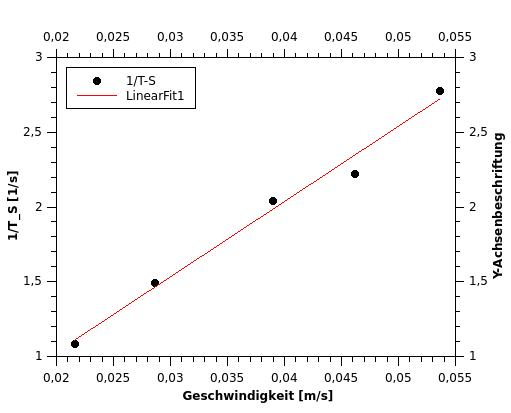
\includegraphics[scale=0.8]{./figure/Aufgabe3_weg_von_Beob.png}
% 	\caption{ Weg von }
% 	\label{fig:weg_von}
% \end{figure}
\end{multicols}
\begin{figure}[H]
	\centering
	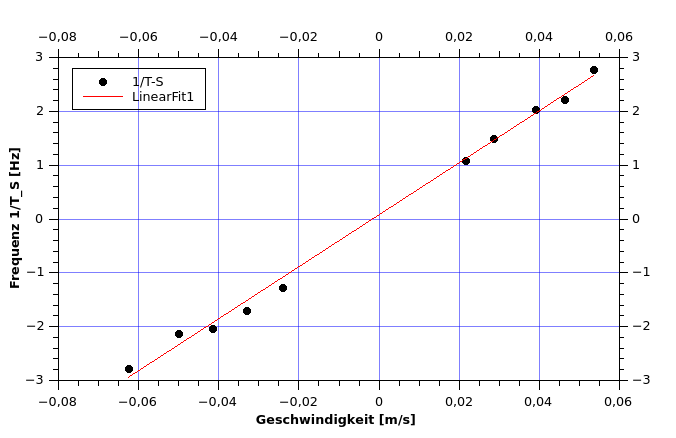
\includegraphics[scale=2.3]{./figure/Dopplereffekt.png}
	\caption{Dopplereffekt lin. Regression mit bewegtem Beobachter in beide Richtungen}
	\label{fig:doppler}
\end{figure}
\begin{multicols}{2}


\pagebreak
%%%%%%%%%%%%%%%%%%%%%%%%%%%%%%%%%%%%%%%%%%%%%%%%%%%%%%%%%%%%%%%%%%%%%%%
\section{Diskussion}
\textbf{Drehpendel}

\textbf{Gekoppelte Pendel}

\textbf{Dopplerverschiebung einer bewegten Schallquelle}


\section{Quellen}
$[1]$ Anleitung, \url{http://www.univie.ac.at/anfpra/neu1/ps/ps1/PS1.pdf}\\
$[2]$ Rohdaten, \url{htts://github.com/blackandcold/Protocols-SS2014-P2/tree/master/PS_1/data}\\

\end{multicols}
\end{document}